\documentclass[CS5104-Notes.tex]{subfiles}
\begin{document}

\section{Basis expansion}

\subsection{Polynomial regression}
To extend linear regression to settings where the function is non-linear, basis functions are used to construct a larger space of functions. A basis function (or number of basis functions) are defined on the input $X$. For example
\begin{equation}
h_{1}(X) = 1, h_{2}(X) = X, h_{3}(X) = X^{2}
\end{equation}
forms three basis functions which is used to transform the input. This transformation replaces the standard linear model
\begin{equation}
f(X) = \theta_{0} + \theta_{1}X
\end{equation}
with new inputs
\begin{equation}
[h_{1}(X), h_{2}(X), h_{3}(X)]^{T} \rightarrow [1,X,X^{2}]^{T}
\end{equation}
to get a polynomial function
\begin{align}
f(X) &= \theta_{0}h_{1}(X) + \theta_{1}h_{2}(X) + \theta_{2}h_{3}(X) \\
 &= \theta_{0} + \theta_{1}X + \theta_{2}X^{2}
\end{align}
Now the same linear regression can be run on the new input as the output is a linear combination of functions, which a linear regression model can still be applied on. The functions may be non-linear, but the input space has been transformed through the non-linear mapping. Of course, this can naturally be extended to $m$ polynomials, but generally using more than 3 or 4 polynomials leads to high chances of overfitting.

\subsection{Piecewise linear regression} Basis expansions are in fact more general than polynomial expansion. Basis functions can also be defined to create a piecewise linear regression model. 

\subsection{Regression splines}
A spline is a piecewise \textit{polynomial} that uses $m + k$ basis functions
\begin{align}
  h_{i}(X) &= X^{i-1}, \forall\ i = 1, 2, ..., m
  h_{m+j}(X) &= (X - \xi_{j})_{+}^{m-1}, \forall\ j = 1, 2, ..., k
\end{align}
where $m$ is th order of the spline + 1, for example a cubic spline is order 4 and $k$ is the number of knots in the piecewise.
\n
The first set of basis functions $h_{i}(X)$ are the normal basis functions for a polynomial expansion while the second set of basis functions $h_{m+j}(X)$ determine the knots. In particular, $\xi_{j}$ determines the location of the $j$th knot. 
\section{Bayesian classification}
In Bayesian terms, input variables are called \textbf{evidence}. The Bayes rule allows the probability and evidence to be expressed into simpler distributions:
\begin{equation}
P(C_{i} | X) = \frac{P(X|C_{i}) P(C_{i})}{P(X)}
\end{equation}
where 
\begin{itemize}
\item $P(C_{i} | X)$ is the \textbf{posterior probability}. In other words, if we know $X$ happened, how likely is $C$?
\item $P(X|C_{i})$ is the \textbf{likelihood}. If we know that the right answer is $C$, how likely is observation $X$?
\item $P(C_{i})$ is the \textbf{prior}, which is how often $C_{i}$ is the correct answer in total. This can often be measured or estimated.
\item $P(X)$ is the \textbf{probability of evidence}, which is how often this particular observation is obtained.
\end{itemize}
Many classifiers attempt to calculate the posterior directly, for example logistic regression. The underlying assumption is that the priors will not change. 
\subsection{Maximum a Posteriori classification}
The maximum likelihood classifier picks the class most likely to generate X. It only makes sense when the classes are approximately equally likely.
\begin{equation}
\hat{Y} = \text{argmax}_{c}P(X|C)
\end{equation}
Next, a maximum a posteriori (MAP) classifier can be defined which maximises the posterior
\begin{equation}
\hat{Y} = \text{argmac}_{c}P(X|C)P(C)
\end{equation}
This allows for easy integration of priors, which can adapt to changing conditions. The probabilities are typically found be the integral of the probability density function.
\begin{figure}[H]
  \centering
  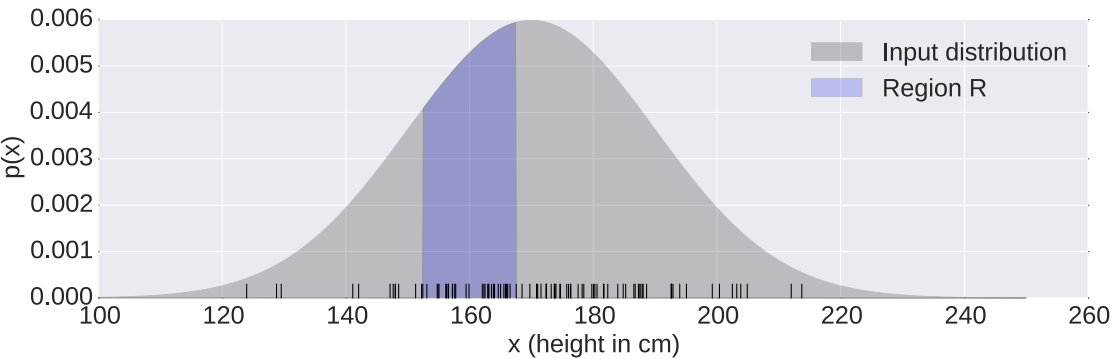
\includegraphics[width=0.9\textwidth, keepaspectratio]{imgs/height-distribution.png}
\end{figure}
\noindent
\begin{equation}
P_{R} = \int_{R}P(X)dX
\end{equation}
Of course, this only applies to distribution of one dimension, where the distribution can be easily calculated and visualised. In distributions of higher dimensions, the probability must be estimated using the local neighbourhood. The idea behind this is \textbf{local density estimation}, where the probability density as position $X$ from the number of samples  $K$ inside a volume $V$
\begin{align}
  X &= [X_{1}, X_{2}, ..., X_{P}]^{T} \\
  p(X) &= \frac{K}{NV}
\end{align}
where $P$ is the number of dimensions and $N$ is the number of samples. The assumption is that density is roughly constant locally. With these assumptions, there are several methods based on this principle, which differ in how they set $K$ and $V$ and how they divide the feature space into subvolumes. 
\begin{figure}[H]
\centering
\begin{subfigure}{0.3\textwidth}
  \centering
  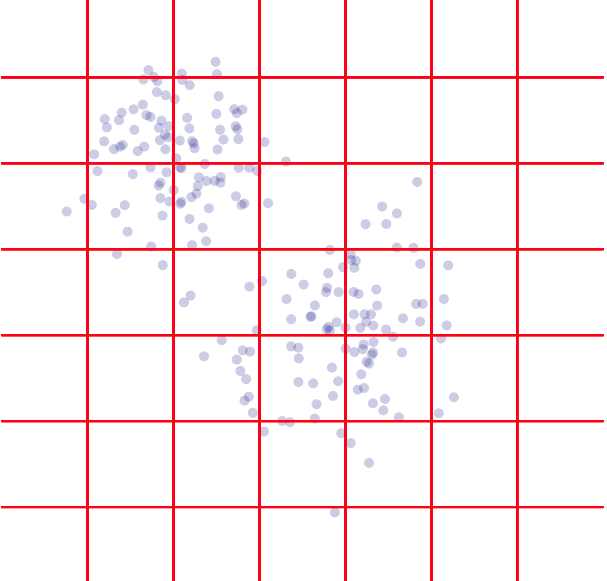
\includegraphics[width=1\textwidth, keepaspectratio]{imgs/histogram-estimation.png}
  \caption{Histogram}
\end{subfigure}
\hspace*{1cm}
\begin{subfigure}{0.3\textwidth}
  \centering
  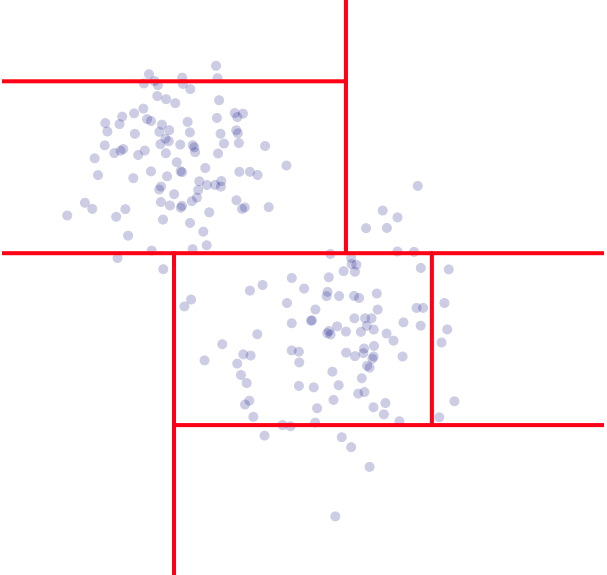
\includegraphics[width=1\textwidth, keepaspectratio]{imgs/decision-tree-estimation.png}
  \caption{Decision tree}
\end{subfigure}
\n
\begin{subfigure}{0.3\textwidth}
  \centering
  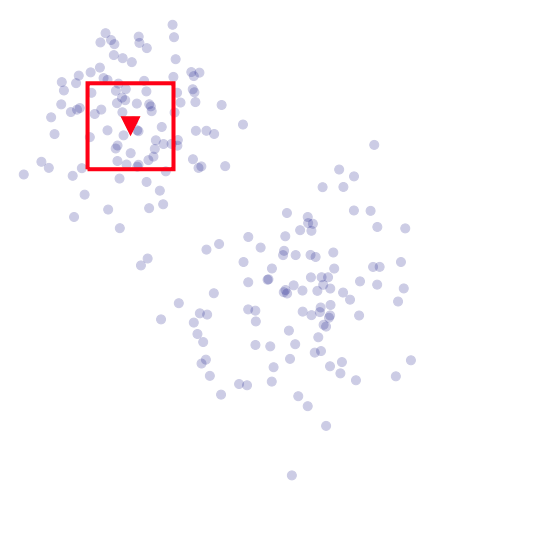
\includegraphics[width=1\textwidth, keepaspectratio]{imgs/tophat-kernel-estimation.png}
  \caption{Tophat kernel}
\end{subfigure}
\hspace*{1cm}
\begin{subfigure}{0.3\textwidth}
  \centering
  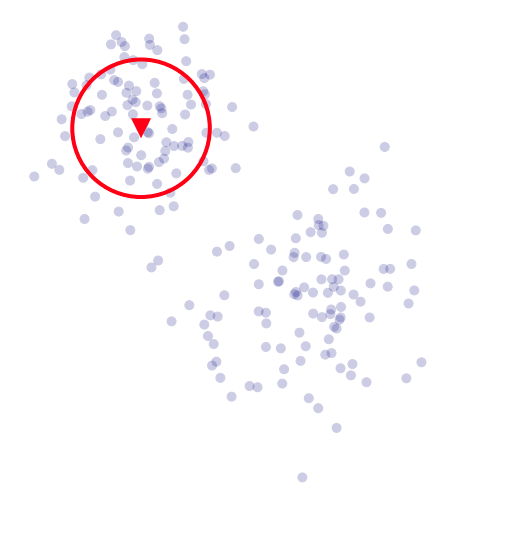
\includegraphics[width=1\textwidth, keepaspectratio]{imgs/knn-estimation.png}
  \caption{kNN}
\end{subfigure}
\end{figure}

\subsubsection{Histograms}
A histogram estimation imposes a strict grid on the feature space, which fixes $V$ while allowing $K$ to vary. This method is very sensitive to the bin size (size of the defined grid) and quite crude.

\subsubsection{Parzen density estimation}
The idea here is to represent the distribution as a sum of statistical \textbf{kernels}.
\begin{equation}
p(X) = \frac{1}{N}\sum_{n=1}^{N}\frac{1}{V}k(\frac{X-x_{N}}{h})
\end{equation}
where $h$ is the bandwidth parameter. The simple example is the \textbf{tophat kernel}
\begin{equation}
k(U) =
\begin{cases}
  1 & |U_{i}| \leq \frac{1}{2}, i = 1, 2, ..., P \\
  0 & \text{otherwise}
\end{cases}
\end{equation}
The distance to each previously seen sample needs to be calculated, which is an expensive computation when there is a lot of data. The advantage gained is no training stage is needed, and there are some efficient data structures which help speed up this process.

\subsubsection{k-Nearest Neighbours}
The kNN algorithm chooses a $K$ value to keep constraint while growing the volume $V$ around the data point $x$ as needed:
\begin{equation}
p(X) = \frac{K}{NV}
\end{equation}
The conditional probabilities by counting data points is generated by each class $C_{i}$
\begin{equation}
p(X | C_{i}) = \frac{K_{i}}{N_{i}V}
\end{equation}
and after applying Bayes' theorem:
\begin{equation}
p(C_{i} | X) = \frac{p(X|C_{i})P(C_{i})}{p(X)} = \frac{K_{i}}{K}
\end{equation}

\subsubsection{Bandwith parameter}
The bandwidth parameter $h$ in the density estimation equations can be varied to control the amount of smoothing. Small values of $h$ will increase the variance (overfit the data) while large values of $h$ will increase the bias (underfit the data). Typically the choice of $h$ is not obvious and it must be found via cross-validation.
\begin{figure}[H]
\centering
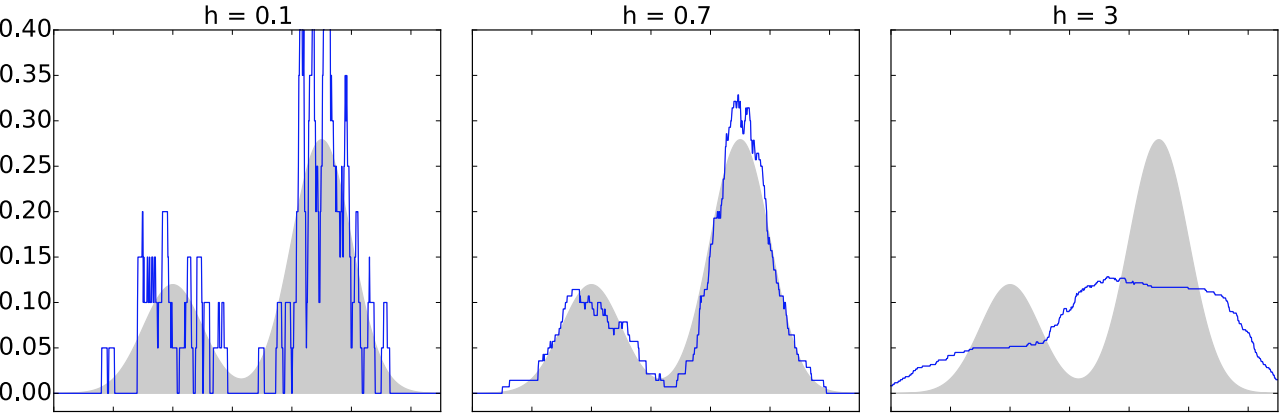
\includegraphics[width=0.8\textwidth, keepaspectratio]{imgs/bandwidth.png}
\caption{The influence of the bandwidth $h$.}
\end{figure}

\section{Support vector machines}

\subsection{Maximal margin classifer}
Recall in logistic regression, there is a decision boundary where data points on one side are classified as a class, and data points on the other side are classified another class. For a problem in $n$-dimensional space, a $n-1$-dimensional hyperplane is defined as the decision boundary. For example in a two-dimensional (x,y) space, the decision boundary is a one-dimensional hyperspace, in other words, a line.
\n
The definition of a hyperplane is quite simple, for example a two-dimensional hyperplane is defined by the equation
\begin{equation}
\beta_{0} + \beta_{1}X_{1} + \beta_{2}X_{2} = 0
\end{equation}
for the parameters $\beta_{0}, \beta_{1}$ and $\beta_{2}$. Any point $X$ in which the equation holds is a point that is on the hyperplane. Of course, the definition is easily extended to a $n$-dimensions:
\begin{align}
  \beta_{0} + \beta_{1}X_{1} + \beta_{2}X_{2} + ... + \beta_{n}X_{n} &= 0 \\
  \beta_{0} + \sum_{i=1}^{n}\beta_{i}X_{i} &= 0
\end{align}
Any point $X = (X1,X2,...,X_{p})^{T}$ that satisfies the equation for the hyperplane lies on the hyperplane. Suppose a point $X$ does not satisfy the equation, and instead,
\begin{equation}
\beta_{0} = \beta_{1}X_{1} + \beta_{2}X_{2} + ... + \beta_{n}X_{n} > 0
\end{equation}
then $X$ lies on one side of the hyperplane. Conversely, if
\begin{equation}
\beta_{0} = \beta_{1}X_{1} + \beta_{2}X_{2} + ... + \beta_{n}X_{n} < 0
\end{equation}
then $X$ lies on the other side of the hyperplane.
\n
This makes a lot of sense for classification problems, as the hyperplane divides the dataset into two halves. It is then also easy to calculate which side of the hyperplane a point lies by calculating the left hand side.
\subsubsection{Classification with a hyperplane}
With a training dataset with data points $x_{1}, x_{2}, ..., x_{n}$ that falls into two classes specified by $y_{1}, y_{2}, ..., y_{n}$. It is observed that the output $y$ variables have the range $\{-1, 1\}$ where -1 represents one class and 1 the other class. Assuming that it is possible to construct a hyperplane that separates the training data points perfectly into the two classes.
\begin{figure}[H]
  \centering
  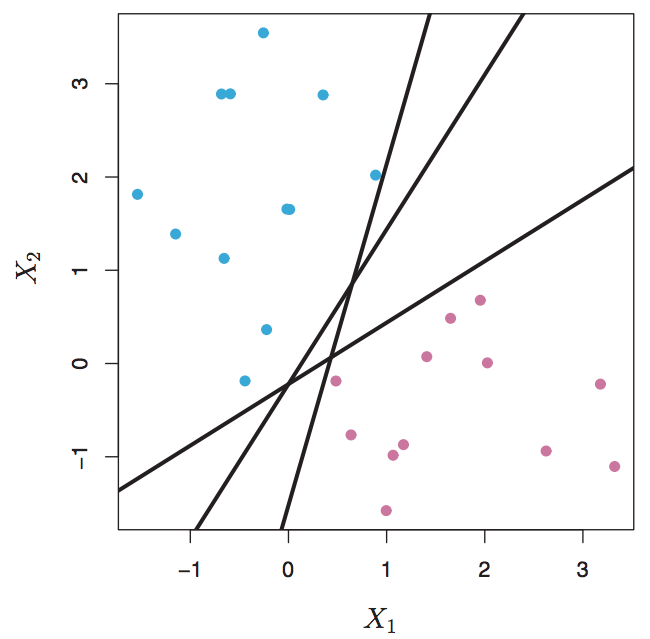
\includegraphics[width=0.4\textwidth, keepaspectratio]{imgs/separating-hyperplanes.png}
  \caption{Example of three separating hyperplanes, out of many possible to perfectly split the blue and purple data points.}
\end{figure}
\noindent
This gives the separating hyperplane has the property that
\begin{align}
  \beta_{0} + \beta_{1}x_{i1} + \beta_{2}x_{i2} + ... + \beta_{n}x_{in} &> 0 \text{ if } y_{i} = 1, \\
  \beta_{0} + \beta_{1}x_{i1} + \beta_{2}x_{i2} + ... + \beta_{n}x_{in} &< 0 \text{ if } y_{i} = -1
\end{align}
for all $i = 1,2,...,n$. In fact, there are infinitely many such hyperplanes that can exist by tweaking the plane slightly up or down, or rotating it slightly without touching any existing data points.
\subsubsection{The maximal margin classifier}
In order to create a classifier based on a separating hyperplane, only one hyerplane should be chosen out of the infinitely possible hyperplanes. A natural choice is the \textbf{maximal margin hyperplane}, which chooses the separating hyperplane that is the farthest away from the training data points. The distance between each training data to a given separating hyperplane can be calculated; the smallest such distance from each class is the minimal distance from the hyperplane and is known as the \textbf{margin}. The maximal margin hyperplane is defined as the separating hyperplane for which the margin is largest, in other words, the hyperplane that has the farthest minimum distance to the training data points. New test data can then be classified based on which side of the hyperplane they lie on. This is a good choice because the large margin means it takes a bigger difference ``jump'' to cross the boundary and lead to a misclassification.
\begin{figure}[H]
  \centering
  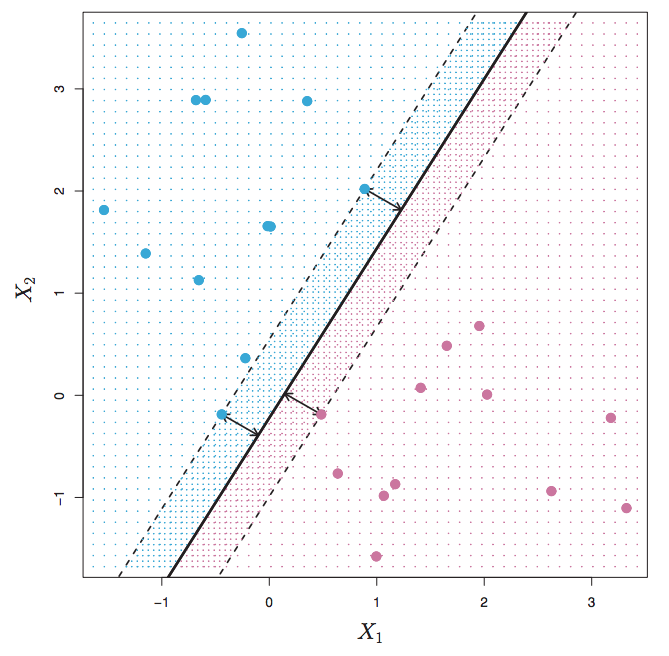
\includegraphics[width=0.4\textwidth, keepaspectratio]{imgs/maximum-margin-hyperplane.png}
  \caption{The maximal margin hyperplane shown which separates the blue and purple data. The three points on the dashed lines that exactly lie at the width of the margin are the support vectors.}
\end{figure}
\noindent
Any points that lie exactly on the width of the margin are known as \textbf{support vectors} as they support the maximal margin hyperplane because if they moved, then the maximal margin hyperplane would move as well. The chosen hyperplane therefore depends directly on these support vectors and not on any other data points unless they move past the margin.
\subsubsection{Maximal margin optimisation problem}
To actually construct the maximal margin hyperplane from the training examples is to find the solution to the following optimisation problem:
\begin{align}
  &\text{maximise} M \\
  &\text{subject to } \sum_{j=1}^{n}\beta_{j}^{2} = 1, \\
  &y_{i}(\beta_{0} + \beta_{1}x_{i1} + ... + \beta_{n}x_{in}) \geq M\ \forall i = 1,2,...,n
\end{align}
The third constraint requires that each training data point be on the correct side of the hyperplane.  The second constraint
\begin{equation*}
\text{subject to } \sum_{j=1}^{n}\beta_{j}^{2} = 1
\end{equation*}
in combination with the third constraint ensures that all training points are on the correct side of the hyperplane \textit{and} are at least a distance $M$ away from the hyperplane.
\n
Of course this would not work for more complicated datasets that are not easily separable, as this only works with the assumption that \textit{a separating hyperplane exists}. If a separating hyperplane does not exist, then the maximal margin classifier cannot be constructed. Furthermore, there is an issue of maximal margin classifiers too easily overfitting to the training data as it is required that the maximal margin hyperplane perfectly split the two sets of data.
\begin{figure}[H]
  \centering
  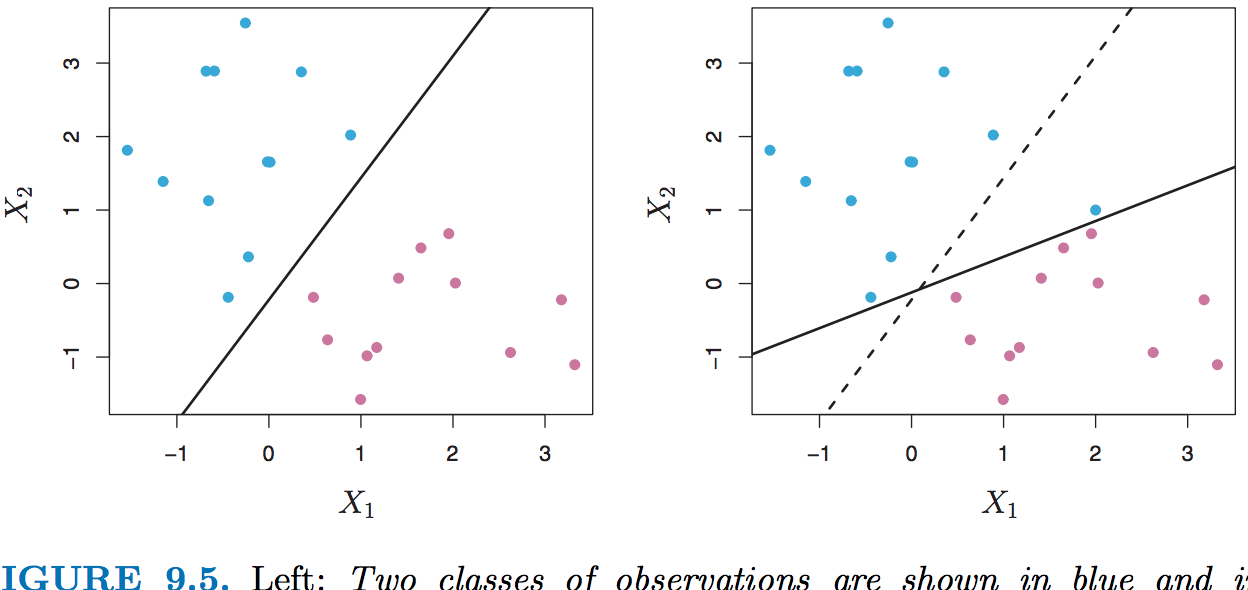
\includegraphics[width=0.9\textwidth, keepaspectratio]{imgs/maximal-margin-problem.png}
  \caption{The addition of another data point on the right leads to a dramatic shift of the maximal margin hyperplane in order to keep the perfect split between the two sets of data.}
\end{figure}

\subsection{Support vector classifiers}
From the observation that a maximal margin classifier does not work for non-separable data and further is highly sensitive to changes in data, the next step is to define a classifier that uses the same concepts of margins, but allows for a hyperplane that does \textit{not} perfectly separate the data. There are two advantages in this approach:
\begin{enumerate}
\item Greater robustness to individual data points
\item Better classification of \textit{most} training data points
\end{enumerate}
In other words, it may be worth misclassifying some samples to increase the generality of the model. This is known as the \textbf{support vector classifier}, or the \textbf{soft margin classifier}. Here, training points are allowed to be on the wrong side of the margin, and even on the wrong side of the hyperplane.
\subsubsection{Support vector optimisation problem}
The optimisation problem from the maximal margin classifier is altered to allow for incorrect classifications. To do so, new slack variables $\epsilon$ are introduced into the optimisation problem
\begin{align}
  &\text{maximise } M \\
  &\text{subject to } \sum_{j=1}^{n}\beta_{j}^{2} = 1, \\
  &y_{i}(\beta_{0} + \beta_{1}x_{i1} + ... + \beta_{n}x_{in}) \geq M(1 - \epsilon_{i}) \\
  &\epsilon_{i} \geq 0, \sum_{i=1}^{n}\epsilon_{i} \leq C
\end{align}
where $C$ is a non-negative tuning parameter. $\epsilon_{1},...,\epsilon_{n}$ are the slack variables that allow individual observations to be on the wrong side of the margin or the hyperplane. The slack variable $\epsilon_{i}$ tells us where the $i$th observation is located relative to the hyperplane and margin.
\begin{itemize}
\item If $\epsilon_{i} = 0$, then the data point is on the correct side of the margin
\item If $\epsilon_{i} > 0$, then the data point is on the wrong side of the margin
\item If $\epsilon_{i} > 1$, then the data point is on the wrong side of the hyperplane
\end{itemize}
The tuning parameter $C$ is important as it bounds the sum of the slack variables. It controls the number and severity of the violations to the margin that are allowed. In other words, it is the amount of tolence that the margin can be violated by $n$ observations. For example, if $C = 0$ then there is no allowance for violations, which is the same as the maximal margin classifier. For any $C > 0$, no more than $C$ observations are allowed on the wrong side of the hyperplane, as $\epsilon_{i} > 1$ if the point is on the wrong side. In practice, $C$ is chosen via cross-validation. As with most tuning parameters, $C$ controls the bias-variance trade-off.
\begin{figure}[H]
\centering
\begin{subfigure}{0.4\textwidth}
  \centering
  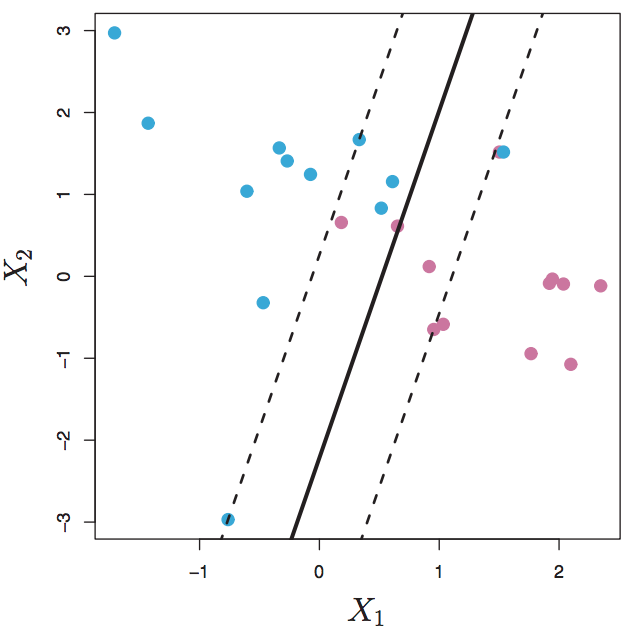
\includegraphics[width=1\textwidth, keepaspectratio]{imgs/support-vector-classification1.png}
\end{subfigure}
\begin{subfigure}{0.4\textwidth}
  \centering
  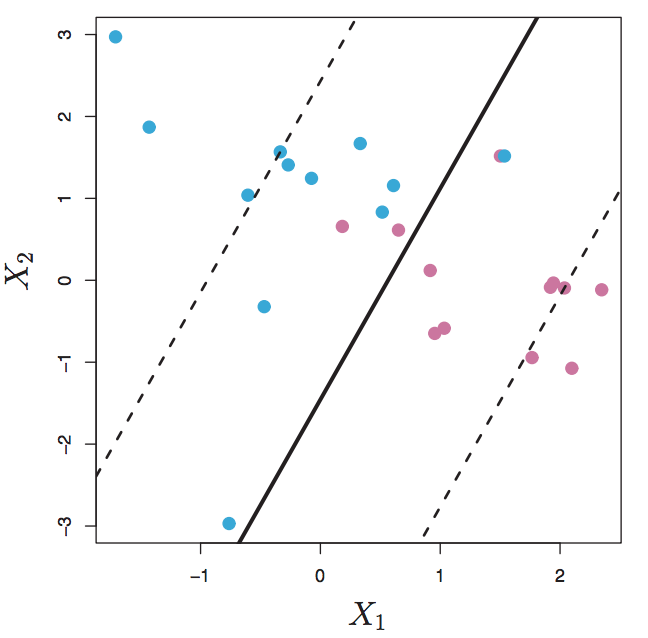
\includegraphics[width=1\textwidth, keepaspectratio]{imgs/support-vector-classification2.png}
\end{subfigure}
\caption{Example of support vector classification with different values for the tuning parameter $C$.}
\end{figure}
\begin{itemize}
\item If $C$ is small, there is less tolerence to data points on the wrong side of the margin and hyperplane, so the classifier is more likely to overfit the data
\item Conversely, if $C$ is large, more violations are allowed, so the classifier has a higher chance of underfitting the data
\end{itemize}
Finally, an interesting point is that only data points within the margins of the classifier affect the hyperplane. Any data points that lie outside the margin have no effect on the hyperplane or classifier just like the maximal margin classifier, where only support vectors affect the classifier. By basing the decision on only a smaller subset of training points that are more likely to affect the behaviour, the method is robust to the behaviour of data far away from the hyperplane. Additional data points not close to the hyperplane do not affect the classifier in any way.

\subsection{Support vector machines}
We have seen how support vector classifiers can allow for data points to lie on the wrong side of the margin and hyperplane and this cost leads to building a more generalisable model. However all these classifiers so far only work with linear-decision boundaries. So the linear classifier must be converted to produce non-linear decision boundaries.

\subsubsection{Non-linear decision boundaries}
In polynomial regression, the same problem of converting a linear regression model to non-linear curves as found. To address the issue in support vector classifiers, the same method can be applied by enlarging the feature space using higher-order polynomial functions of the predictors. For example, instead of fitting the support vector classifier with $n$ features
\begin{equation*}
X_{1}, X_{2}, ..., X_{n}
\end{equation*}
$2n$ features with a quadratic function can be used instead
\begin{equation*}
X_{1}, X_{1}^{2}, X_{2}, X_{2}^{2}, ..., X_{n}, X_{n}^{2}
\end{equation*}
Although the decision boundary found in the enlarged feature space is still linear, it is non-linear in the original feature space as it is in the form $q(x) = $ where $q$ is a quadratic or higher-order polynomial. However, this has the issue of creating too many features for a high number of polynomials.
\subsubsection{Priaml and dual optimisation problem}
The support vector optimisation problem
\begin{align*}
  &\text{maximise } M \\
  &\text{subject to } \sum_{j=1}^{n}\beta_{j}^{2} = 1, \\
  &y_{i}(\beta_{0} + \beta_{1}x_{i1} + ... + \beta_{n}x_{in}) \geq M(1 - \epsilon_{i}) \\
  &\epsilon_{i} \geq 0, \sum_{i=1}^{n}\epsilon_{i} \leq C
\end{align*}
can be turned into an objective function by \textbf{Lagrange relaxation}
\begin{equation}
  L_{P} = \frac{1}{2}||\beta||^{2} + C\sum_{i=1}^{n}\epsilon_{i}
  - \sum_{i=1}^{n}\alpha_{i}[y_{i}(x_{i}^{T}\beta + \beta_{0}) - (1 - \epsilon_{i})]
  - \sum_{i=1}^{n}\mu_{i}\epsilon_{i}
\end{equation}
where $C$, $\alpha_{i}$ and $\mu_{i}$ are lagrange multipliers, which serve as a substitute for hard constraints and must be positive. This objective function is called the \textbf{primal} problem.
\begin{itemize}
\item $\frac{1}{2}||\beta||^{2}$ maximises the margin by minimising $||\beta||$
\item $C\sum_{i=1}^{n}\epsilon_{i}$ is the tolerance for violations of the margin and hyperplane
\item $\sum_{i=1}^{n}\alpha_{i}[y_{i}(x_{i}^{T}\beta + \beta_{0}) - (1 - \epsilon_{i})]$ punishes errors as the expression becomes negative if a data point is on the wrong side of the margin
\item $\sum_{i=1}^{n}\mu_{i}\epsilon_{i}$ makes $\epsilon_{i}$ positive by punishing negative values
\end{itemize}
The primal problem is difficult to optimise for. The constraints are implicit rather than hard and violations are allowed, but punished, which follows from the soft margin classifier of allowing violations. The primal problem can be transforms into the \textbf{dual problem} which is easier to solve. This is done by differentiating with respect to $\beta, \beta_{0}$ and $\epsilon_{i}$, which gives
\begin{align}
  \beta &= \sum_{i=1}^{n}\alpha_{i}y_{i}x_{i} \\
  0 &= \sum_{i=1}^{n}\alpha_{i}y_{i} \\
  \alpha_{i} &= C - \mu_{i}
\end{align}
These values can be put back into the primal function to give the dual function
\begin{equation}
L_{D} = \sum_{i=1}^{n}\alpha_{i} - \frac{1}{2}\sum_{i=1}^{n}\sum_{i'=1}^{n}\alpha_{i}\alpha_{i'}y_{i}y_{i'}x_{i}^{T}x_{i'}
\end{equation}
which is easier to put into a standard solver.

\subsubsection{Support vector classifier solution}
By solving the primal or dual functions, the solution to the support vector classifier can be found. It turns out that the solutions only involves the \textit{inner product} of the data points, defined as
\begin{equation}
\langle x_{i}, x_{i'} \rangle = \sum_{j=1}^{n}x_{ij}x_{i'j}
\end{equation}
The support vector classifier can then be represented as
\begin{equation}
f(x) = \beta_{0} + \sum_{i=1}^{p}\alpha_{i}\langle x,x_{i} \rangle
\end{equation}
where there are $p$ parameters $\alpha_{i}$ per training example. To esimate the parameters, all that is needed is the dot product of the training pair $\langle x,x_{i} \rangle$. Although this means that to evaluate the function $f(x)$, the dot product must be computed for each new point $x$ and every existing training point $x_{i}$. However, $\alpha_{i}$ is only nonzero for support vectors, so a lot of computation can be saved by only computing the functions for the set of support vectors rather than every single training point.
\n
In summary, only the dot product $\langle x,x_{i} \rangle$ is needed in computing the coefficients of the linear classifier $f(x)$.
\subsubsection{Kernel trick}
Now the trick to extend the support vector classifier to a support vector machine that works on non-linear data is to replace the dot product with a \textit{generalisation} in the form
\begin{equation}
K(x_{i},x_{i'})
\end{equation}
where $K$ is some kernel function. This is very similar to basis expansions as the kernel $K$ defines a basis function to apply on $x_{i}$ and $x_{i'}$.
\begin{equation}
K(x_{i},x_{i'}) = \langle h(x_{i}),h(x_{i'}) \rangle
\end{equation}
where $h$ is the basis expansion. There are many common kernels that can be used, including the original linear kernel,
\begin{itemize}
\item Linear kernel
  \begin{equation}
    K(x_{i}, x_{i'}) = \sum_{j=1}^{n}x_{ij}x_{i'j}
  \end{equation}
\item Polynomial kernel where $d$ is the polynomial degree
  \begin{equation}
    K(x_{i}, x_{i'}) = (1 + \sum_{j=1}^{n}x_{ij}x_{i'j})^{d}
  \end{equation}
\item Radial kernel
  \begin{equation}
    K(x_{i}, x_{i'}) = \text{exp}(\gamma \sum_{j=1}^{n}(x_{ij} - x_{i'j})^{2})
  \end{equation}
\end{itemize}
\begin{figure}[H]
\centering
\begin{subfigure}{0.4\textwidth}
  \centering
  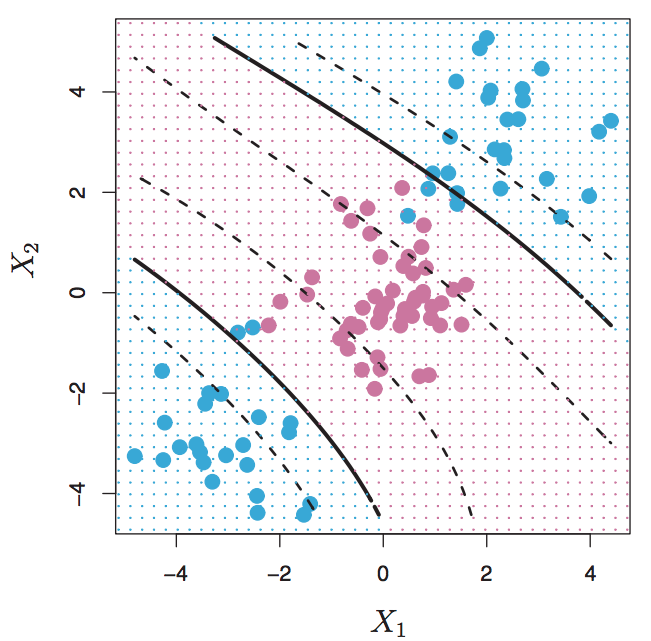
\includegraphics[width=1\textwidth, keepaspectratio]{imgs/polynomial-kernel.png}
  \caption{SVM with a polynomial kernel of degree 3}
\end{subfigure}
\hspace*{\fill}
\begin{subfigure}{0.4\textwidth}
  \centering
  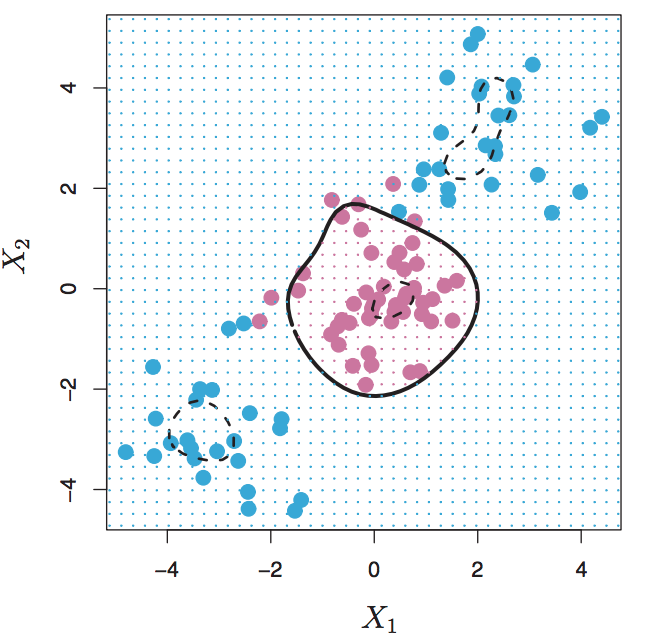
\includegraphics[width=1\textwidth, keepaspectratio]{imgs/radial-kernel.png}
  \caption{SVM with a radial kernel}
\end{subfigure}
\end{figure}

\subsection{Hinge loss function}
It turns out that SVMs have a close connection to logistic regression. The optimisation problem for SVMs can be rewritten in the form
\begin{equation}
J(\beta) = \frac{1}{N}\sum_{i=1}^{n}(1 - y_{i}(x_{i}^{T}\beta + \beta_{0})) + \lambda \sum_{j=1}^{n}\beta_{j}^{2}
\end{equation}
where
\begin{itemize}
\item $J(\beta)$ is the cost function
\item $(1 - y_{i}(x_{i}^{T}\beta + \beta_{0}))$ is the \textbf{hinge loss}
\item $\lambda \sum_{j=1}^{n}\beta_{j}^{2}$ is the regularisation
\end{itemize}
This function looks very similar to the functions for logistic regression, but using a hingle loss function rather than a squared error loss. Further, the regularisation term $\lambda \sum_{j=1}^{n}\beta_{j}^{2}$ is the same as a ridge $l_{2}$ norm in linear regression.
\n
The difference between support vector classification, which uses the hinge loss, and logistic regression, which uses a squared error loss is the data points that are on the correct side of the margin do not affect the classifier. This comes from the hinge loss characteristic where the loss function is exactly zero when $y_{i}(\beta_{0} + \sum_{j=1}^{n}\beta_{j}x_{ij}) /geq 1$, corresponding to data points on the right side of the margin. In contrast, the loss function for logistic regression is never zero, though it can be very small for data points that are far away.
\end{document}


